\documentclass[a4paper]{article}
\def\DOCTITLE{CSC3423 Biocomputing}
% Set document attributes
\title{\DOCTITLE}

\usepackage{fullpage}
\usepackage{scrextend}
\usepackage{titlesec}
\usepackage{fancyhdr}
\usepackage{amsmath}
\usepackage{amssymb}

% Handle graphics correctly
\ifx\pdftexversion\undefined
\usepackage{graphicx}
% \usepackage[dvips]{graphicx}
\else
\usepackage[pdftex]{graphicx}
\DeclareGraphicsRule{*}{mps}{*}{}
\fi

% Setup headers and footers
\pagestyle{fancy}
\lhead{}
\chead{\DOCTITLE}
\rhead{}
\rfoot{}
\cfoot{\thepage}
\lfoot{}

% New page for each section
% \newcommand{\sectionbreak}{\clearpage}

% Set header and footer sizes
\renewcommand{\headrulewidth}{0.4pt}
\renewcommand{\footrulewidth}{0.4pt}
\setlength{\headheight}{15.2pt}
\setlength{\headsep}{15.2pt}

\setlength{\parskip}{5pt plus 1pt minus 1pt}
\setlength{\parindent}{0pt}

\newcommand{\Forall}{\;\forall\;}
\newcommand{\Mod}{\: mod \:}


\begin{document}

\tableofcontents

\section{Overview}
\label{sec:overview}

\begin{table}[h]
  \centering
  \begin{tabular}{@{}l|cccccc@{}}
    \toprule
    Problem Type     & GA/GP/MA     & NN          & ACO           & PSO         & CA          & MC          \\
    \midrule
    Optimisation     & \checkmark   &             & (\checkmark)  & \checkmark  &             &             \\
    Machine Learning & \checkmark   & \checkmark  & (\checkmark)  & \checkmark  &             &             \\
    Control          & \checkmark   & \checkmark  & (\checkmark)  & \checkmark  &             &             \\
    Simulation       & (\checkmark) &             &               &             & \checkmark  & \checkmark  \\
    \bottomrule
  \end{tabular}
  \caption{Suitability of algorithms to problems}
  \label{tab:suitability}
\end{table}

\begin{description}
  \item[GA]   Genetic Algorithm
  \item[GP]   Genetic Programming
  \item[MA]   Memetic Algorithm
  \item[NN]   Neural Network
  \item[ACO]  Ant Colony Optimisation
  \item[PSO]  Particle Swarm Optimisation
  \item[CA]   Cellular Automata
  \item[MC]   Membrane Computing
\end{description}

\section{Genetic Algorithms}
\label{sec:ga}

\subsection{Biological Inspiration}

\Para{Natural selection}

Principle that every slight change in a trait that is beneficial is preserved.

Individuals that have traits that allow them to be better adapted to the
environment are more likely to reproduce, traits are then passed to later
generations.

\Para{Genetics}

Candidate solutions to a problem represented in a chromosome composed of several
genes.

Genes are passed from generation to generation with small changes (mutations).

\subsection{Overview}

\begin{figure}[h!]
  \centering
  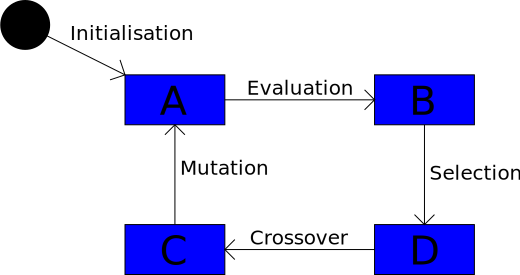
\includegraphics[width=0.5\textwidth]{out/ga_workflow.eps}
  \caption{Genetic Algorithm Workflow}
  \label{fig:ga_workflow}
\end{figure}
\FloatBarrier

\Para{Pseudocode}

\begin{listing}[h]
  \begin{minted}{python}
    population = init_random_population()
    iteration = 0
    while iteration < num_interations:
      evaluate(population)
      population = selection(population)
      population = crossover(population)
      population = mutation(population)
      iteration++
    best = get_best_individual(population)
    return best
  \end{minted}
  \caption{Genetic algorithm pseudocode}
  \label{listing:ga_pseudocode}
\end{listing}

\subsection{Population}

\begin{itemize}
  \item Set of possible solutions to the problem
  \item Most often a set (chromosome) of variables (genes)
  \item Initial population created at random
\end{itemize}

\subsection{Evaluation}

\begin{itemize}
  \item Giving a "goodness" value to each candidate solution
  \item Uses a fitness function which takes a candidate solution and determines
        how well it solves the problem
\end{itemize}

\subsection{Selection}

\begin{itemize}
  \item Choosing individuals to be in the next population
  \item Rewards best individuals (i.e. those with the best fitness values)
\end{itemize}

\subsubsection{Roulette Wheel Selection}

\begin{itemize}
  \item Probability of selection is proportional to fitness of individual
  \item Make as many selections (spins of wheel) as individuals to be selected
  \item Individuals may be selected multiple times
\end{itemize}

\begin{figure}[h!]
  \centering
  \includegraphics[width=0.4\textwidth]{out/roulette_wheel_selection.eps}
  \caption{Roulette Wheel Selection}
  \label{fig:roulette_wheel_selection}
\end{figure}
\FloatBarrier

\subsubsection{Stochastic Universal Sampling}

\begin{itemize}
  \item Similar to Roulette Wheel Selection
  \item Do one spin but divide "pointer" into as many individuals to be selected
\end{itemize}

\begin{figure}[h!]
  \centering
  \includegraphics[width=0.4\textwidth]{out/stochastic_universal_sampling.eps}
  \caption{Stochastic Universal Sampling}
  \label{fig:stochastic_universal_sampling}
\end{figure}
\FloatBarrier

\subsubsection{Tournament Selection}

\begin{itemize}
  \item Select the best individual from a randomly selected subset of the
        population
\end{itemize}

\begin{listing}[h]
  \begin{minted}{python}
    new_population = []
    while population.size() > 0:
      tournament = select_random_subset(population, tournament_size)
      tournament = sort_by_fitness(tournament)
      new_population.add(tournament[0])
    return new_population
  \end{minted}
  \caption{Tournament selection pseudocode}
  \label{listing:ga_tournament_selection_pseudocode}
\end{listing}

\subsubsection{Truncation Selection}

\begin{itemize}
  \item Keep only the best $n$ individuals in a population
\end{itemize}

\subsubsection{Comparison of selection methods}

\begin{description}
  \item[Roulette Wheel \& Stochastic Selection] \hfill \\
    \begin{itemize}
      \item Fitness proportionate
      \item Chance of being selected is proportionate to fitness value
      \item Selection becomes random when fitness values are close (e.g. in
            later GA iterations)
    \end{itemize}

  \item[Tournament \& Truncation Selection] \hfill \\
    \begin{itemize}
      \item Rank based
      \item Best individual will always win a tournament
      \item More stable selection pressure
    \end{itemize}

\end{description}

\subsection{Crossover}

\begin{itemize}
  \item Exchanging genes between two individuals
  \item Takes two individuals from the population and generates two offspring
  \item e.g. For a bit array, one offspring takes first section of array and
        second of another, and vice-versa
  \item e.g. For numerical genes the blend alpha operator picks a random value
        between the two parent genes
\end{itemize}

\subsection{Mutation}

\begin{itemize}
  \item Making small/subtle modifications to an individual
  \item Probability $P_{m}$ of mutation can be set either per chromosome or per
        individual
  \item e.g. Randomly flipping a bit where the chromosome is a bit array
  \item e.g. Adding a random value to a numerical gene
\end{itemize}

\subsection{Replacement}

\begin{itemize}
  \item Alternative to generational genetic algorithm
  \item Steady state genetic algorithm
    \begin{itemize}
      \item Elitism
      \item Selection chooses two parents who produce two offspring
      \item Offspring are inserted into the parent population, replacing the
            two individuals with lowest fitness
    \end{itemize}
\end{itemize}

\subsection{Knowledge Representation}

Nominal attributes:

\begin{itemize}
  \item Set of rules and logic predicates
\end{itemize}

Real valued attributes:

\begin{itemize}
  \item Hyperrectangle ($n$ dimension rectangle)
  \item Hyperellipsoid ($n$ dimension circle)
  \item Decision trees
  \item Synthetic prototypes (e.g. nearest neighbour)
  \item Linear classifier (separate instances of classes for classification
        problems)
\end{itemize}

\begin{figure}[h]
  \centering
  \begin{subfigure}[b]{0.4\textwidth}
    \includegraphics[width=\textwidth]{out/kr_decision_tree.eps}
    \caption{Decision Tree}
  \end{subfigure}
  \begin{subfigure}[b]{0.4\textwidth}
    \includegraphics[width=\textwidth]{out/kr_nearest_neighbour.eps}
    \caption{Nearest Neighbour}
  \end{subfigure}
  \caption{}
  \label{fig:ga_knowledge_representations}
\end{figure}
\FloatBarrier

\subsection{Tuning}

\begin{itemize}
  \item Required to ensure a proper evolutionary process
  \item GA learns well when exploration and exploitation are balanced
    \begin{description}
      \item[Exploration]
        Directing population to unknown areas of the problem space
      \item[Exploitation]
        Directing the population to most promising (based on fitness) parts of
        the problem space
    \end{description}
  \item Too much exploitation can lead to convergence to a sub-optimal solution
        (premature convergence)
    \begin{itemize}
      \item If population is too similar then crossover operator no longer
            provides effective exploration
    \end{itemize}
  \item Too much exploration risks:
    \begin{itemize}
      \item Slowing down the learning process
      \item If probabilities are too high then crossover and mutation may harm
            the overall population fitness
    \end{itemize}
  \item Innovation time $t_{i}$ is the average time taken to create an
        individual with better fitness than the current best individual
\end{itemize}

\subsection{Machine Learning}

\begin{description}
  \item[Supevised learning] \hfill \\
    \begin{itemize}
      \item Learning to solve a problem
      \item If output is discrete \RArrow Classification (output value known as
            a class)
      \item If output is continuous \RArrow Regression
      \item Use a training set to train the genetic algorithm and a testing set
            to verify the generated model
      \item Optimise initialisation by creating initial population based on
            training data
    \end{itemize}

  \item[Unsupervised learning] \hfill \\
    \begin{itemize}
      \item Identifying patters/clusters
    \end{itemize}

\end{description}

\subsection{Parallel Genetic Algorithms}

\begin{itemize}
  \item Genetic algorithms tend to be slow
  \item Majority of genetic operations can be parallelised (all but crossover)
  \item Several systems exist for this:
    \begin{description}
      \item[Master-Slave model]
        GA cycle is is run on master, slaves perform operations
      \item[Island Model]
        Population is divided across nodes
      \item[Cellular GA]
        Population distributed across 2D lattice
    \end{description}
\end{itemize}

\section{Genetic Programming}
\label{sec:gp}

\begin{itemize}
  \item Very similar concept to Genetic Algorithms \ref{sec:ga}
  \item Instead of evolving a solution, evolve a program

\end{itemize}

\subsection{Program Representation}

\begin{itemize}
  \item Classic method is to represent programs as a tree representing a
        formula
  \item Modern methods can also create other representations
    \begin{itemize}
      \item e.g. Cartesian Genetic Programming creates graphs
    \end{itemize}
  \item Internal nodes of tree are functions/operations
  \item Leaves are either variables/parameters or constants
    \begin{itemize}
      \item Constants can be predefined or assigned a random value within a
            predefined range
    \end{itemize}
\end{itemize}

\Para{Example}

Figure \ref{fig:gp_tree_example} shows a tree representing the equation:
\[
  \frac{4 + P3}{P1 - sin(P2)}
\]

\begin{figure}[h!]
  \centering
  \includegraphics[width=0.3\textwidth]{out/gp_tree_example.eps}
  \caption{Example Tree}
  \label{fig:gp_tree_example}
\end{figure}
\FloatBarrier

\subsection{Initialisation}

\begin{itemize}
  \item Initial tree is generated randomly
  \item Maximum depth of tree is predefined
  \item Strategies for generation:
    \begin{description}
      \item[Grow] \hfill \\
        Generate a tree at random with leaves up to the maximum depth
      \item[Fill] \hfill \\
        Generate a tree at random with all leaves at the maximum depth
      \item[Hybrid] \hfill \\
        For each level of depth, initialise a uniform number of trees, half of
        which using Grow and half using Full
    \end{description}
\end{itemize}

\begin{figure}[h]
  \centering
  \begin{subfigure}[t!]{0.4\textwidth}
    \includegraphics[width=0.5\textwidth]{out/gp_tree_grow.eps}
    \caption{Grow}
  \end{subfigure}
  \begin{subfigure}[t!]{0.4\textwidth}
    \includegraphics[width=0.8\textwidth]{out/gp_tree_fill.eps}
    \caption{Fill}
  \end{subfigure}
  \caption{Tree initialisation}
  \label{fig:gp_initialisation}
\end{figure}
\FloatBarrier

\subsection{Evaluation/Execution}

\begin{itemize}
  \item Evaluation is done by averaging error over all test cases, giving a
        fitness value
  \item Recursive execution is easy but inefficient
  \item Converting a tree to Reverse Polish Notation solves problem
\end{itemize}

\begin{listing}[h]
  \begin{minted}{text}
    for each element e:
      if e is value:
        push e to the stack
      else if e is operator:
        pop as many elements from the stack as the operator has parameters
        execute the operator
        push the result to the stack
    return value at top of stack
  \end{minted}
  \caption{Genetic programming execution pseudocode}
  \label{listing:gp_eval_pseudocode}
\end{listing}

\subsection{Crossover}

Exchange subtrees between parents.

\Para{Example}

\begin{figure}[h]
  \centering
  \begin{subfigure}[t!]{0.4\textwidth}
    \includegraphics[width=0.8\textwidth]{out/gp_tree_example.eps}
  \end{subfigure}
  \begin{subfigure}[t!]{0.4\textwidth}
    \includegraphics[width=0.8\textwidth]{out/gp_tree_example_mutation.eps}
  \end{subfigure}
  \caption{Tree crossover parents}
  \label{fig:gp_crossover_parents}
\end{figure}
\FloatBarrier

\begin{figure}[h]
  \centering
  \begin{subfigure}[t!]{0.4\textwidth}
    \includegraphics[width=0.8\textwidth]{out/gp_tree_child_1.eps}
  \end{subfigure}
  \begin{subfigure}[t!]{0.4\textwidth}
    \includegraphics[width=0.8\textwidth]{out/gp_tree_child_2.eps}
  \end{subfigure}
  \caption{Tree crossover children}
  \label{fig:gp_crossover_children}
\end{figure}
\FloatBarrier

\subsection{Mutation}

Replace entire subtrees with a randomly generated subtree.

\Para{Example}

\begin{figure}[h]
  \centering
  \begin{subfigure}[t!]{0.4\textwidth}
    \includegraphics[width=0.8\textwidth]{out/gp_tree_example.eps}
    \caption{Before}
  \end{subfigure}
  \begin{subfigure}[t!]{0.4\textwidth}
    \includegraphics[width=0.8\textwidth]{out/gp_tree_example_mutation.eps}
    \caption{After}
  \end{subfigure}
  \caption{Tree mutation}
  \label{fig:gp_mutation}
\end{figure}
\FloatBarrier

\subsection{Bloat}

\begin{itemize}
  \item Growth of program tree without improvement in fitness
  \item Bloat can affect any evolutionary paradigm where the representation
        has variable length
  \item Solutions:
    \begin{description}
      \item[Restrict tree depth] \hfill \\
        May affect evolutionary process making it unable to find a good
        solution
      \item[Simplification] \hfill \\
        Very difficult to do efficiently
      \item[Add fitness penalty to large trees] \hfill \\
        Smaller fitness for solutions with larger trees
      \item[Consider tree size in selection] \hfill \\
        When two individuals have equal fitness, prefer the smaller tree
    \end{description}
\end{itemize}

\subsection{Applications}

\begin{description}
  \item[Regression] \hfill \\
    Reverse engineering a mathematical formula given a dataset of output values
    for given input values.

    This gives an approximation of the original formula that created the
    dataset.

  \item[Generating Electronic Circuits] \hfill \\
    Tree topology defines schematic.

    Leaves define component values (inductance, capacitance, etc.).

  \item[Control] \hfill \\
    Optimising gains of a PID controller.

  \item[Puzzle Solvers] \hfill \\
    e.g. FreeCell solver using hybrid genetic algorithm and genetic
    programming.

  \item[Generation of Audio Synhesizers] \hfill \\
    Using Cartesian Generic Programming to generate a graph structure.

\end{description}

\section{Neural Networks}
\label{sec:nn}

\begin{itemize}
  \item Connection of perceptrons
  \item Perceptron
    \begin{itemize}
      \item Set of inputs from other perceptrons
      \item Activation/transfer function
      \item Output value
    \end{itemize}
  \item Connection
    \begin{itemize}
      \item Weighted
    \end{itemize}
  \item Used for data problems (classification, regression, control)
\end{itemize}

\begin{figure}[h!]
  \centering
  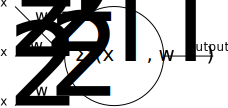
\includegraphics[width=0.5\textwidth]{out/perceptron.eps}
  \caption{Perceptron}
  \label{fig:perceptron}
\end{figure}
\FloatBarrier

\subsection{Multi Layer Perceptron}

\begin{itemize}
  \item Multi layer neural network where every perceptron in a layer is
        connected to every neuron in the adjacent layers
    \begin{itemize}
      \item A single input layer with as many neurons as they are input
            parameters
      \item Several inner layers
      \item A single output layer with as many neurons as they are outputs
    \end{itemize}
  \item Each layer represents a combination of features
    \begin{itemize}
      \item e.g. phonemes -> words -> sentences
    \end{itemize}
  \item A non linear multi layer perceptron with a single inner layer with
        enough neurons can learn any continuous function (universal
        approximation theory)
\end{itemize}

\begin{figure}[h!]
  \centering
  \includegraphics[width=0.5\textwidth]{out/multi_layer_perceptron.eps}
  \caption{Multi Layer Perceptron}
  \label{fig:multi_layer_perceptron}
\end{figure}
\FloatBarrier

\subsubsection{Learning Task}

\begin{itemize}
  \item Supervised learning given a set of inputs and the expected output
  \item Optimise the error function \ref{eq:mlp_e} to obtain the smallest value
        of $E$ by selecting new values of the weights $W$
  \item Computationally difficult to do using traditional optimisation methods
        (e.g. steepest-descent, Newton, etc.)
  \item Classic method for MLP is using backpropagation algorithm
    \begin{itemize}
      \item Two pass approach
      \item Calculate error of output layer
      \item Calculate weight updates of next layer back in turn
    \end{itemize}
\end{itemize}

\begin{align}
  E &= \frac{1}{n} \sum^{n}_{t=1} E(x')                   \\
    &= \frac{1}{n} \sum^{n}_{t=1} (F(x', W) - y_{t})^{2}
  \label{eq:mlp_e}
\end{align}

\subsection{Self Organised Maps}

\begin{itemize}
  \item a.k.a Kohonen neural network
  \item Unsupervised neural network
  \item Maps data from a high dimensionality to a 2D lattice
\end{itemize}

\begin{figure}[h!]
  \centering
  \includegraphics[width=0.8\textwidth]{out/som_training.eps}
  \caption{Self Organising Map Training}
  \label{fig:som_training}
\end{figure}
\FloatBarrier

Training:

\begin{enumerate}
  \item[1] A new input vector is selected
  \item[2] The node with a weight vector closest to the input vector (best
           matching unit) is found
  \item[3] The weight vector of the BMU and it's neighbours is modified to
           bring them closer to the input vector
\end{enumerate}

\subsection{Deep Learning}

\begin{itemize}
  \item A neural network with lots ($\geq 10$) inner layers
  \item More inner layers allows construction/recognition of higher level
        features
\end{itemize}

Types:

\begin{itemize}
  \item Purely supervised (deep NN)
    \begin{itemize}
      \item Trained using classic methods (e.g. backpropagation)
      \item Results in very slow training times due to network size
    \end{itemize}

  \item Semi-supervised (deep belief networks)
    \begin{itemize}
      \item Build inner layers incrementally in an unsupervised way
      \item Add a final supervised layer
    \end{itemize}

  \item Generative methods (convolutional NN)
    \begin{itemize}
      \item Each layer applies a "filter" to the data to reduce its
            dimensionality
      \item Commonly used with image/signal processing
    \end{itemize}
\end{itemize}

\subsubsection{Training semi-supervised networks}

\begin{enumerate}
  \item[1] Train first layer in an unsupervised manner
  \item[2] Fix first layer parameters and train second layer using the output of
           the first layer as unsupervised input to the second
  \item[3] Repeat for all inner layers
  \item[4] Use the outputs of the final layer as inputs to a supervised layer
           and train using the raining data outputs
  \item[5] Free all parameters and train entire network using a supervised
           approach using existing weights as initial values
\end{enumerate}

\subsubsection{Restricted Boltzmann machine}

\begin{itemize}
  \item Unsupervised neural network that learns a probability distribution over
        a set of inputs
  \item The result is it will learn to recognise recurrent patterns
\end{itemize}

\subsubsection{Convolutional Neural Network}

\begin{itemize}
  \item Each layer combines "patches" from the previous layer
  \item Compresses larger problems into smaller sets of features
  \item Filters are usually manually defined (i.e. not learned)
  \item Output of filtering is used to train a supervised model
  \item Requires neighbourhood regularity in input data (i.e. areas of a certain
        colour in an image)
\end{itemize}

\section{Memetic Algorithms}
\label{sec:ma}

\begin{itemize}
  \item Derived form the concept of traits spreading from person to person
  \item Combines conventional genetic algorithm (global search) with local
        search
  \item Global search allows exploration of entire problem space
  \item Local search allows exploration of neighbourhood of each individual to
        attempt to improve its fitness
\end{itemize}

\Para{Pseudocode}

\begin{listing}[h]
  \begin{minted}{python}
    population = init_random_population()
    iteration = 0
    while iteration < num_interations:
      evaluate(population)
      for i in range(len(population)):
        population[i] = select_local_best(population[i])
      population = selection(population)
      population = crossover(population)
      population = mutation(population)
      iteration++
    best = get_best_individual(population)
    return best
  \end{minted}
  \caption{Memetic algorithm pseudocode}
  \label{listing:ma_pseudocode}
\end{listing}

\subsection{Motivation}

\begin{itemize}
  \item When decomposing complex problems, subproblems may be easier to solve
        using either GA or local search
  \item Fast to reach optimal solution using domain specific knowledge in local
        search operator
  \item Domain knowledge in local search operator can "repair" bad individuals
        found by a GA
\end{itemize}

\subsection{Design considerations}

\Para{Baldwinism vs Lamarckism}

Two alternative theories for transfer of traits between individuals of a
population.

\begin{description}
  \item[Baldwinism] \hfill \\
    \begin{itemize}
      \item Traits acquired by an individual can be passed to its offspring
      \item e.g. replace an individual with its fitter neighbour
    \end{itemize}

  \item[Lamarckism] \hfill \\
    \begin{itemize}
      \item Traits acquired by an individual cannot be passed to its offspring
      \item e.g. individual inherits fitness but not genotype
    \end{itemize}

\end{description}

\Para{When to apply local search?}

\begin{itemize}
  \item After selection
  \item After crossover
  \item After mutation
\end{itemize}

\Para{In which stage of the genetic algorithm lifecycle?}

\begin{itemize}
  \item Uniformly throughout all iterations
  \item More in earlier or later iterations
\end{itemize}

\Para{Scope of local search?}

\begin{itemize}
  \item Entire population
  \item Probability of local search (fitness proportionate)
  \item Only individuals with specific range of fitness values
\end{itemize}

\Para{Choice of local search operator}

\begin{itemize}
  \item Use multiple, each of which having a fixed probability of being applied
  \item Have a fixed mapping of individuals to operator (domain specific)
  \item Evolve the operator choice using a GA
\end{itemize}

\Para{Other design issues}

\begin{itemize}
  \item Size of neighbourhood for local search
  \item Size of variations to make during local search operation
\end{itemize}

\Para{Diversity control}

\begin{itemize}
  \item Memetic algorithms naturally favour exploitation over exploration
  \item To ensure good evolution additional exploration must be done
  \item One option is to increase local search neighbourhood
\end{itemize}

\section{Swarm Intelligence}
\label{sec:swarm}

\begin{itemize}
  \item System of "items" collaborating to solve a task
  \item No external guidance/arbitration/synchronisation
\end{itemize}

\subsection{Ant Colony Optimisation}

\begin{itemize}
  \item Key concept is stigmergy, the indirect communication between individuals
        in the system through the environment
  \item In ants this is done though a pheromone trail deposited by ants as they
        explore a path
  \item Ants will always prefer to follow the path with the strongest pheromone
        trail
  \item Can be applied to any problem assuming it can be represented as a graph
    \begin{itemize}
      \item e.g. Ant-Miner: An unsupervised machine learning framework that
            constructs rules that identify patters in a set of input data.
    \end{itemize}
\end{itemize}

\subsubsection{Example: Travelling Salesperson Problem}

Close problem to actual ant colony movement.

\begin{itemize}
  \item Graph $G(N, E)$: $N$ are cities and $E$ are routed between cities
  \item $d_{i,j}$ is the fixed cost of travelling between cities $i$ and $j$
  \item Edge cost is given by a combination of:
    \begin{enumerate}
      \item[1] Static cost: $\eta(r, s) = \frac{1}{d_{r,s}}$
      \item[2] Dynamic trace: $\tau(r, s)$ deposited by ants (initially zero)
    \end{enumerate}
  \item All ants must visit all nodes in an iteration (a tour)
  \item At the end of an iteration all edges that are on the best tour receive
        additional pheromone
  \item At each iteration the pheromone count for all nodes may be reduced to
        reduce the chances of unpopular edges being selected in a tour
  \item Stopping criteria is either stagnation or a maximum number of iterations
    being performed.
\end{itemize}

\Para{Pseudocode}

\begin{listing}[h]
  \begin{minted}{python}
    graph = init_graph(d)
    place_ants()
    while not stopping_criteria:
      while not all_cities_visited:
        for a in ants:
          move_to_next_city(a)
      place_ants()
      graph = update_graph(tau)
    return graph
  \end{minted}
  \caption{Ant colony optimisation for TSP pseudocode (single iteration)}
  \label{listing:msco_for_tsp_pseudocode}
\end{listing}
\FloatBarrier

\subsection{Particle Swarm Optimisation}

TODO

\section{Cellular Automata}
\label{sec:ca}

TODO

\section{Membrane Computing}
\label{sec:membrane}

TODO

\section{DNA Computing}
\label{sec:dna}

TODO

\end{document}
